\documentclass[../main.tex]{subfiles}

\begin{document}
	\section{Light}
	\begin{preamb}
		Light can be studied as a wave. In this chapter we will look at how light interacts with matter.
	\end{preamb}
	
	\pdef{Normal}{The normal is an imaginary line draw perpendicular to the surface that reflection is taking place at.}
	
	\pdef{Angle of Incidence}{The angle of incidence is the angle between the incident ray and the normal.}
	
	\pdef{Angle of Reflection}{The angle of reflection is the angle between the reflected ray and the normal.}
	
	\begin{center}
		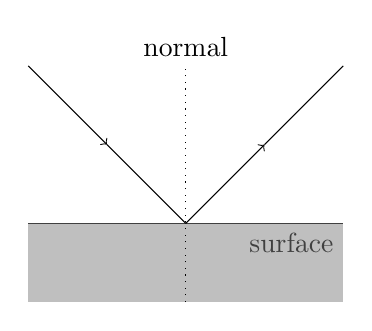
\begin{tikzpicture}
			\draw (-2,0) -- (2,0) node [anchor=north east] {surface};
			\fill [color=gray, fill opacity=0.5] (-2,-1) -- (-2,0) -- (2,0) -- (2, -1);
			\draw [dotted] (0,-1) -- (0,2) node [anchor=south] {normal};
			\draw [->] (-2,2) -- (-1,1);
			\draw (-1,1) -- (0,0);
			\draw [->] (0,0) -- (1,1);
			\draw (1,1) -- (2,2);
		\end{tikzpicture}
	\end{center}
	
	\subsection{Reflection}
	\pdef{Law of Reflection}{In reflection, the angle of incidence is equal to the angle of reflection. The incident ray, reflected ray, and the normal are coplanar. \[\theta_1 = \theta_2\]}
	I have chosen to name the angles \(\theta_1\) and \(\theta_2\) due to the reversible nature of light. It does not matter which way the light goes; the angles will be preserved.
\end{document}
